\documentclass[../TDE7_ocrsf.tex]{subfiles}%

\begin{document}
\section[s]"2"{Résonance d'un circuit bouchon}

\enonce{%
	\begin{minipage}{0.55\linewidth}
		On considère le circuit $RLC$ représenté ci-contre, composé d'un
		résistor, de résistance $R$, d'une bobine idéale d'inductance $L$,
		d'un condensateur idéal, de capacité $C$, alimenté par une source
		idéale de tension, de f.e.m. $e(t)=E_0\cos(\wt)$. On se place en
		régime sinusoïdal forcé.
	\end{minipage}
	\hfill
	\begin{minipage}{0.45\linewidth}
		\begin{center}
			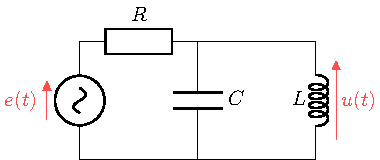
\includegraphics[width=\linewidth]{bouchon_plain}
		\end{center}
	\end{minipage}
}

\QR{%
	Exprimer l'amplitude complexe $\xul{U}$ de $u(t)$ en
	fonction de $E_0$, $R$, $L$, $C$ et $\w$.
}{%
	On effectue un pont diviseur de tension aux bornes de l'impédance
	équivalente de $L$ et $C$, avec $\Yu\ind{eq} = \jcw + 1/\jlw$~:
	\begin{gather*}
		\Uu
		= \frac{\Zu\ind{eq}}{\Zu\ind{eq} + R}E_0
		= \frac{1}{1+R\Yu\ind{eq}}E_0
		= \frac{E_0}{1+\jj \left( RC\w - \dfrac{R}{L\w} \right)}
	\end{gather*}
	en utilisant que $1/\jj = -\jj$.
}

\QR{%
	Établir qu'il existe un phénomène de résonance pour la tension
	$u(t)$. Préciser la pulsation $\w_0$ à laquelle ce phénomène se
	produit et la valeur de l'amplitude réelle de $u(t)$ à cette
	pulsation.
}{%
	L'amplitude réelle est
	\begin{gather*}
		U = \abs{\Uu} = \frac{E_0}{\sqrt{1 + \left( RC\w - \dfrac{R}{L\w}
				\right)^2}}
	\end{gather*}
	Cette tension réelle est maximale si le dénominateur est minimal, donc
	si $\DS \left( RC\w - \frac{R}{L\w} \right) = 0$~: cela implique qu'il y
	a résonance si $\boxed{\w = \w_0 = 1/\sqrt{LC}}$. On trouve alors
	\begin{gather*}
		\boxed{U(\w_0) = U_{\max} = E_0}
	\end{gather*}
}

\QR{%
	Mettre l'amplitude réelle $U$ de $u(t)$ sous la forme: \[U =
		\dfrac{E_0}{\sqrt{1 + Q^2\left(\dfrac{\w}{\w_0} -
				\dfrac{\w_0}{\w}\right)^2}}\] avec $Q$ un facteur sans
	dimension à exprimer en fonction de $R,L$ et $C$.
}{%
	On cherche $Q\w_0 = \frac{R}{L}$ et $\DS\frac{Q}{\w_0} = RC$~; on
	trouve donc
	\[\boxed{Q = R \sqrt{\frac{C}{L}}}\]
}

\QR{%
	Exprimer la bande passante $\Delta\w$ de cette résonance en
	fonction de $Q$ et $\w_0$.
}{%
	On cherche donc les pulsations de coupure telles que $U(\w) =
		\frac{U_{\max}}{\sqrt{2}}$, soit
	\begin{gather*}
		U(\w) = \frac{U_{\max}}{\sqrt{2}}
		\Leftrightarrow
		\frac{E_0}{\sqrt{1 + Q^2\left( \frac{\w}{\w_0} - \frac{\w_0}{\w}
				\right)^2}}
		=
		\frac{E_0}{\sqrt{2}}
		\Leftrightarrow
		\boxed{Q^2\left( \frac{\w}{\w_0} - \frac{\w_0}{\w} \right)^2 = 1}
	\end{gather*}
	On prend la racine carrée de cette équation, \textbf{en prenant les deux
		solutions possibles}~:
	\begin{align*}
		Q\left( \frac{\w}{\w_0} - \frac{\w_0}{\w} \right) = -1
		         & \qet
		Q\left( \frac{\w}{\w_0} - \frac{\w_0}{\w} \right) = 1          \\
		\Leftrightarrow
		\left( \frac{\w}{\w_0} - \frac{\w_0}{\w} \right)\times \w\w_0 =
		- \frac{\w\w_0}{Q}
		         & \qet
		\left( \frac{\w}{\w_0} - \frac{\w_0}{\w} \right)\times \w\w_0 =
		\frac{\w\w_0}{Q}                                               \\
		\Leftrightarrow
		\w^2 - \w_0{}^2 = -\frac{\w\w_0}{Q}
		         & \qet
		\w^2 - \w_0{}^2 = \frac{\w\w_0}{Q}                             \\
		\Leftrightarrow
		\boxed{
			\w^2 + \frac{\w_0}{Q}\w - \w_0{}^2 = 0}
		         & \qet
		\boxed{
		\w^2 - \frac{\w_0}{Q}\w - \w_0{}^2 = 0}                        \\
		\Rightarrow
		\Delta = & \frac{\w_0{}^2}{Q} + 4\w_0{}^2                      \\
		\Leftrightarrow
		\Delta = & \frac{\w_0{}^2}{Q^2} \left( 1 + 4Q^2 \right)        \\
		\Rightarrow
		\w_{1,\pm} = -\frac{\w_0}{2Q} \pm \frac{\w_0}{2Q} \sqrt{1+4Q^2}
		         & \qet
		\w_{2,\pm} = \frac{\w_0}{2Q} \pm \frac{\w_0}{2Q} \sqrt{1+4Q^2} \\
		\Leftrightarrow
		\w_{1,\pm} = \frac{\w_0}{2Q} \left(-1 \pm \sqrt{1+4Q^2}\right)
		         & \qet
		\w_{2,\pm} = \frac{\w_0}{2Q} \left(1 \pm \sqrt{1+4Q^2}\right)
	\end{align*}
	De ces quatre racines, seules deux sont positives~: la solution avec $-1 -
		\sqrt{1+4Q^2}$ est évidemment négative, et celle avec $1 - \sqrt{1+4Q^2}$
	également. Ainsi, il ne nous reste que
	\begin{gather*}
		\w_1 = \frac{\w_0}{2Q} \left( \sqrt{1+4Q^2}-1 \right)
		\qet
		\w_1 = \frac{\w_0}{2Q} \left( \sqrt{1+4Q^2}+1 \right)
	\end{gather*}
	Il ne reste qu'à calculer la différence pour avoir la bande passante~:
	\begin{gather*}
		\boxed{\D\w = \w_2 - \w_1 = \frac{\w_0}{Q}}
	\end{gather*}
}

\QR{%
	En déduire les valeurs numériques de $C$ et $E_0$ à l'aide du
	graphe ci-dessous représentant l'amplitude réelle de $u(t)$ en
	fonction de la fréquence $f=\w/2\pi$, sachant que $L= \SI{1}{mH}$ et
	$R= \SI{1}{k\Omega}$.
	\begin{center}
		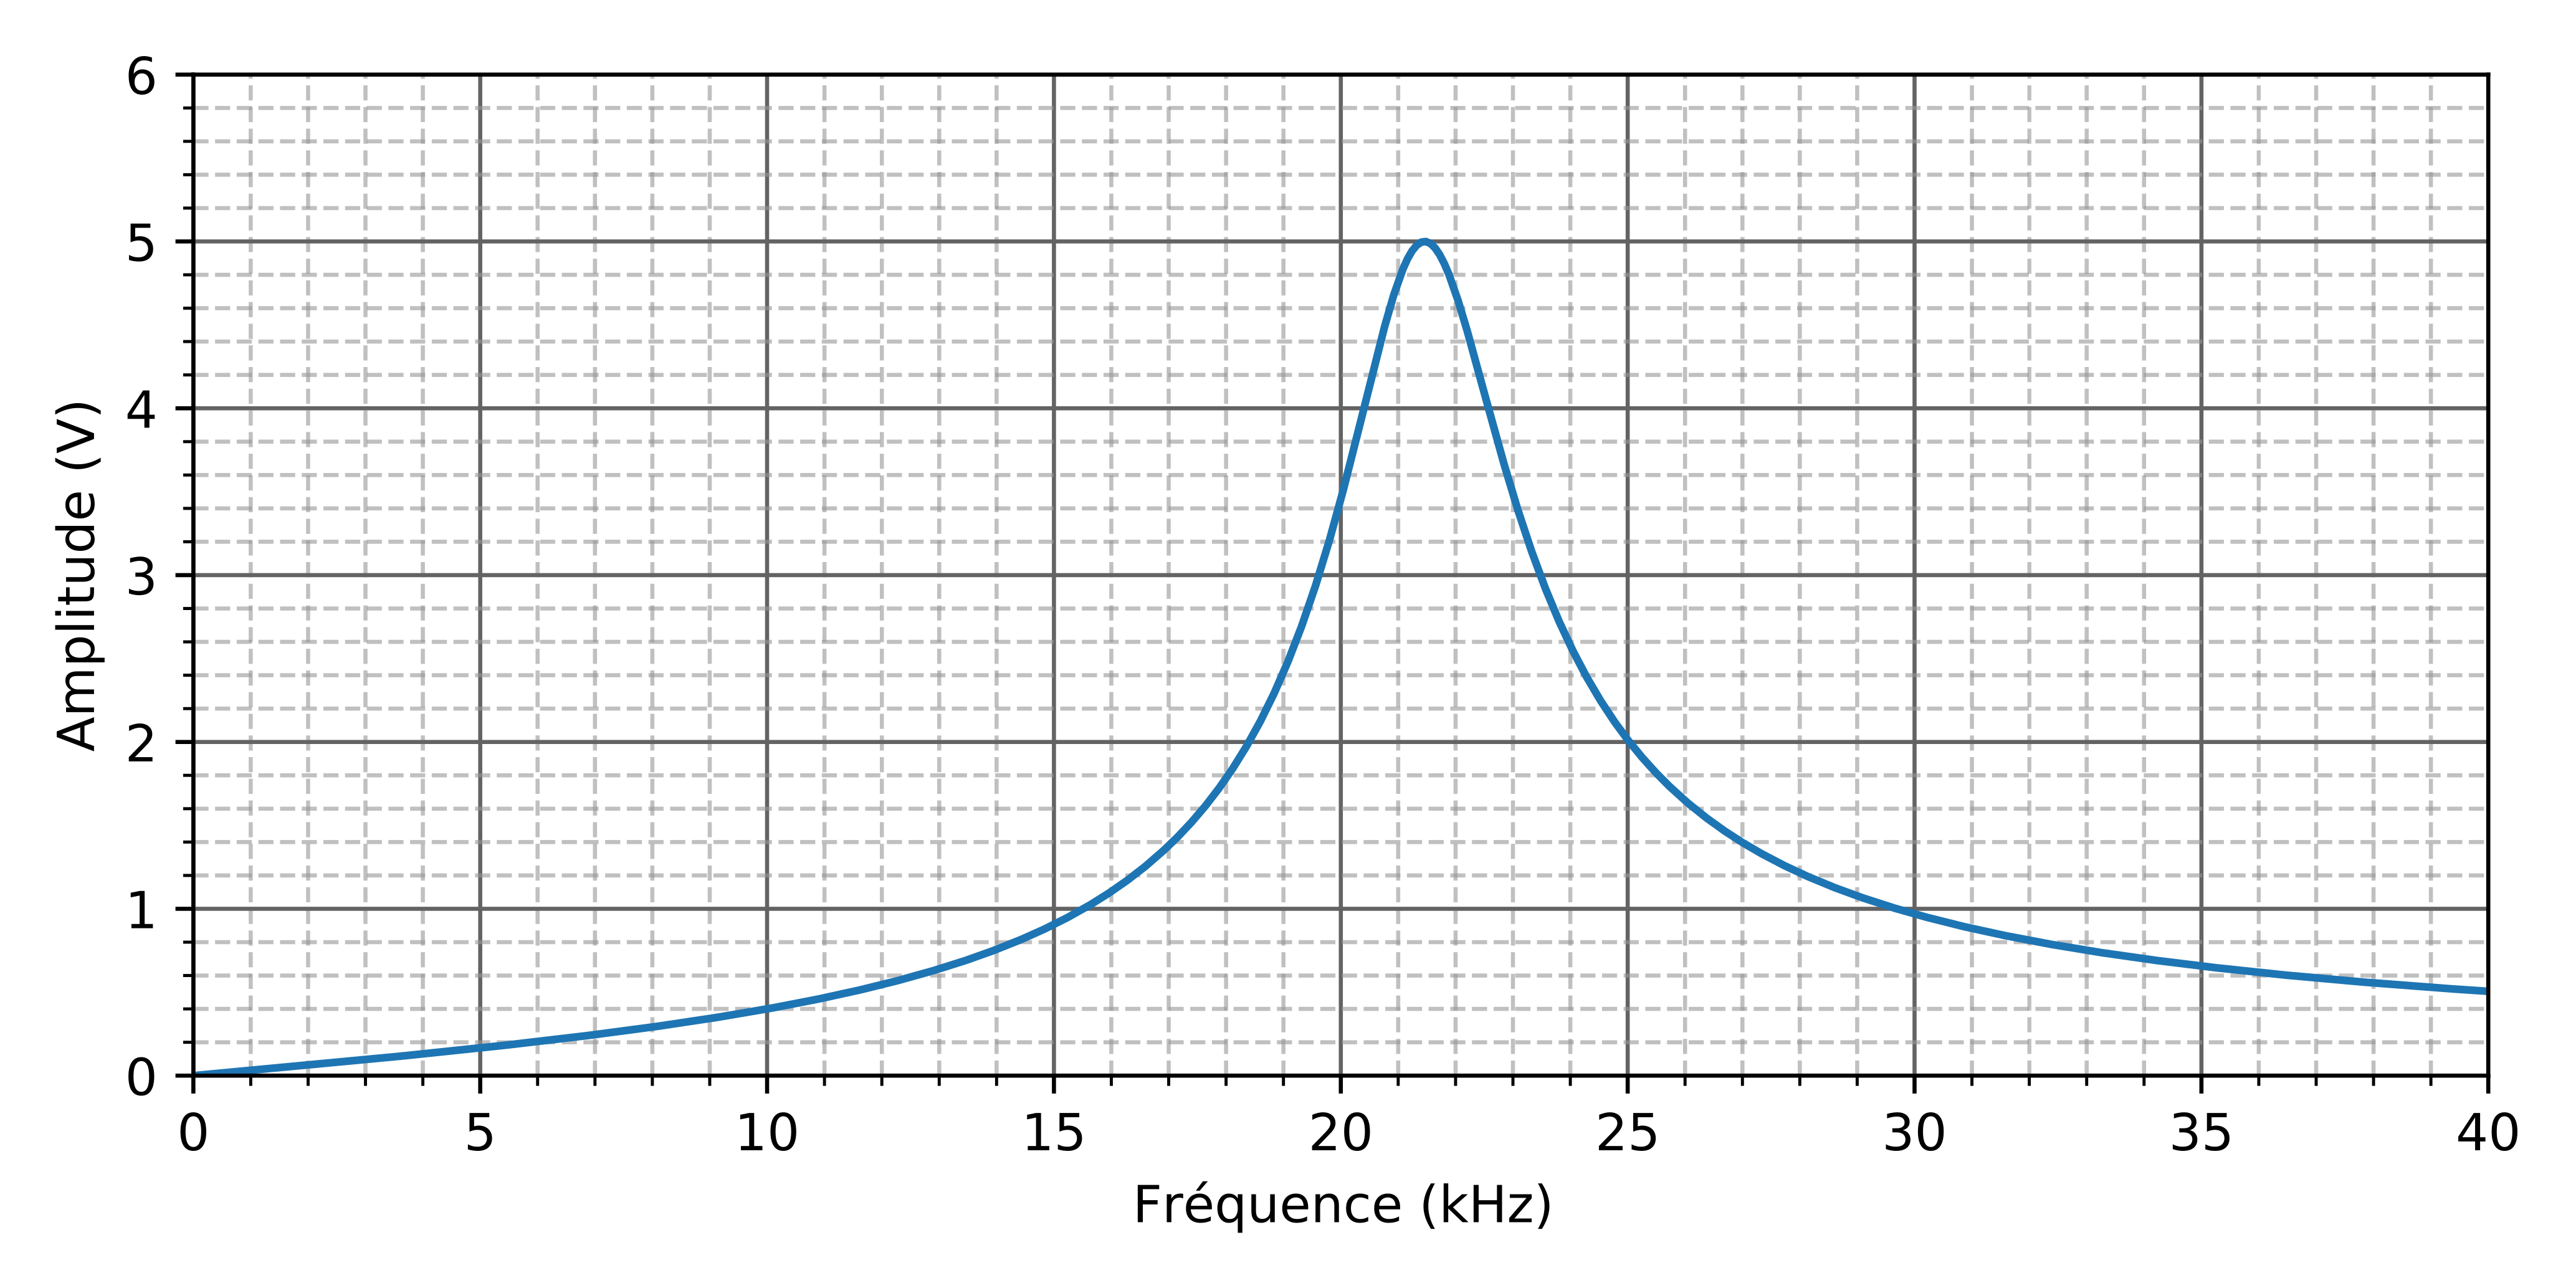
\includegraphics[width=.8\linewidth]{bouchon_2}
	\end{center}
}{%
	Sur le graphique, on trouve $U_{\max} = \SI{5}{V} = E_0$. On a de plus
	$f_0 = \SI{22.5}{kHz}$ et $\D f \approx \SI{3}{kHz}$, d'où $\boxed{Q =
			\frac{f_0}{\D f} \approx \num{7.5}}$. Avec l'expression de $Q$, on isole
	$C$~:
	\begin{gather*}
		Q = R \sqrt{\frac{C}{L}}
		\Leftrightarrow
		\boxed{C = \frac{Q^2L}{R}}
		\qavec
		\left\{
		\begin{array}{rcl}
			Q & = & \num{7.5}       \\
			L & = & \SI{1}{mH}      \\
			R & = & \SI{1}{k\Omega}
		\end{array}
		\right.\\
		\mathrm{A.N.~:}\quad
		\boxed{C = \SI{5.6e-8}{F}}
	\end{gather*}
}
\end{document}
